\chapter{Preliminary making}

%In this chapter I will 

%thought experiments using the horn torus

%Visualizing integration–disintegration trajectories on a horn torus

%anticipatory design of database query using the horn torus


%experiments to test computational information management of a hyperlinked research database


%experiments to test topic modelling between semantic fields for interdisciplinary knowledge translation


%experiments to test more ecological local AI


%observations about information management practices in the University

%..
%In this chapter, I will present my thought experiments visualizing integration-disintegration trajectories on a horn torus, anticipatory design of database query using the horn torus, experiments to test computational information management of a hyperlinked research database, experiments to test topic modelling between semantic fields for interdisciplinary knowledge translation, experiments to test more ecological AI, and last, I offer observations about information management practices in the University. 


\section{Thought experiments using the horn torus}
\index[terms]{torus}
\index[terms]{composition}

This chapter documents the preliminary making, which scaffolds my main thesis contributions: horn-torus thought experiments for integration–disintegration, a toroidal anticipatory query design, a coded query test of a hyperlinked research knowledgebase, testing cross-domain topic modelling for knowledge translation, tests toward more ecological AI, and closing observations on the knowledge stewardship for climate resilience.

\clearpage


\subsection{Visualizing integration–disintegration trajectories on a horn torus}

\begin{figure}[h]
    \centering
    \includegraphics[width=0.5\linewidth]{figures/4.1.png}
    \caption[Visualization of the Horn Torus Semantic Form as a flow of re-creation]
    {\textbf{Visualization of the Horn Torus Semantic Form as a flow of re-creation.} This model of my thought experiment traces the paths of integration from chaos into a `Fullness of being', then back out to 'Potential for being', or complete dis-integration.}
    \label{f4.1}
\end{figure}
\FloatBarrier
\index[terms]{Horn Torus Semantic Form}
\index[terms]{torus}
\index[terms]{composition}

Considering the semantic complexity afforded by Rucker’s torus space-time model, I used the horn torus to visuospatialize cycles of metaphysical and ontological cycles of being. In a sense, I sought to examine the flux between what is and what might be before what is. Lines depict points of a being's journey in relation to the recurring central origin point of \autoref{f4.1}, the `Fullness of being.' Out from this central point arcs the movement through `Disintegration' to dis-integrated chaos as `Potential for being.' The `Integration' arc moves back to `Fullness of being', and so on. The orientation of the horn torus calls back to the trumpet form of a flower as its top hemisphere, and the roots of a plant pulling nutrients from the soil, or disintegrated raw matter, as the bottom hemisphere. The themes of disintegration and integration echo what Ignatius called ``consolation and desolation” \citep{loyola_spiritual_1522,loyola_ejercicios_1548,loyola_spiritual_1914}. I apply these concepts in \autoref{f4.3}, replacing `Disintegration' and `Integration' with `Desolation' and 'Consolation', respectively.
\index[people]{Ignatius of Loyola}
\index[terms]{torus}
\index[people]{Rucker, Rudy} 
\index[terms]{torus}
\index[terms]{horn torus}
\index[terms]{composition}

\FloatBarrier

\begin{figure}[h!]
    \centering
    \includegraphics[width=\linewidth]{figures/4.3 Horn Torus and Sculpture.png} 
    \caption[Horn torus sculpture as Semantic Form information physicalization of consolation and desolation]{\textbf{Horn torus sculpture as Semantic Form information physicalization of consolation and desolation}. \textit{Left}: Horn Torus Semantic Form. \textit{Right}: \textit{Schrödinger’s Theology} (2022), made of foraged Kentucky Coffee Tree branches and unbleached cotton thread.}
    \label{f4.3}
\end{figure}
\FloatBarrier
\index[terms]{Horn Torus Semantic Form}



%\begin{figure}[h]
%    \centering
%    \includegraphics[width=0.5\linewidth]{figures/4.2.png}
%    \caption[Visualization of the horn torus Semantic Form as a cycle of %consolation and desolation]{Visualization of the horn torus Semantic Form %as a cycle of consolation and desolation. This model is the basis of %my artwork \textit{Schrödinger’s Theology} (2022)}
%    \label{f4.2}
%\end{figure}
%If we were to consider the point cloud as a static state of individual points, I endeavoured to illustrate the motion of said points and trace their trajectory across time. 




\subsection{Anticipatory design of database query using the horn torus}
Considering the semantic and semiotic range of the horn torus, I considered how it might be applied to information composition for multiple texts in a larger database. In \autoref{f4.4}, I imagined how a cloud of horn tori might model a database as a heatmap for a researcher’s query, pointing to which texts are most relevant for them. 
\index[terms]{torus}
\index[terms]{horn torus}
\index[terms]{composition}

The horn torus’s negative space at the top and bottom of itself is in the form of two trumpet shapes. If a series of horn tori were attached to each other across their top and bottom openings, they would form a sequence of double cones, resembling the popular double diamond shape used by the British Design Council \citep{british_design_council_framework_nodate}. The similarity in the form could allow for a similar approach to modelling information from a given database in sequences of divergence and convergence; and, perhaps, also sequences of induction and deduction. 
\index[terms]{torus}
\index[terms]{horn torus}

Furthermore, the cone composition appears in significant information visualizations, including Taylor’s cones of plausibility \citep[p. 14]{taylor_creating_1990}, Bezold and Hancock’s futures cone \citep[p. 73]{bezold_overview_1993}, as well as Grant and Booth's meta-analysis funnel plot in their typology of literature reviews \citep[p. 94-95]{grant_typology_2009}.
\index[people]{Bezold, Clement}
\index[terms]{composition}

In \autoref{f4.5}, I propose an example of how isomorphologies in a text network graph can be revealed with Horn Torus Semantic Forms across multiple graphs: (a) the heatmap format would allow for quick identification of the zones most relevant to a Query Isomorph. (b) Heatmaps would also identify through-lines across graphs. 
\index[terms]{network graph} 
\index[terms]{Semantic Forms}
\index[terms]{torus}

Point clouds reveal relationships between points through proximity, distance, and movement, but I was curious about the potential of other forms of visualizing points in space. Network graphs also use individual points but include the addition of lines connecting said points. To examine how information visualization could be applied to large groups of texts, I turned to the emerging space of Personal Knowledge Management (PKM) and platforms like Obsidian, which visualized databases as network graphs.
\index[terms]{Personal Knowledge Management (PKM)} 
\index[terms]{network graph}

\FloatBarrier
\begin{figure}[h]
    \centering
    \includegraphics[width=0.7\linewidth]{figures/4.4.png}
    \caption[Field of horn tori as point plot heatmap with negative space as a sequence of double cones]{\textbf{Field of horn tori as point plot heatmap with negative space as a sequence of double cones.}}
    \label{f4.4}
\end{figure}

\begin{figure}[h]
    \centering
    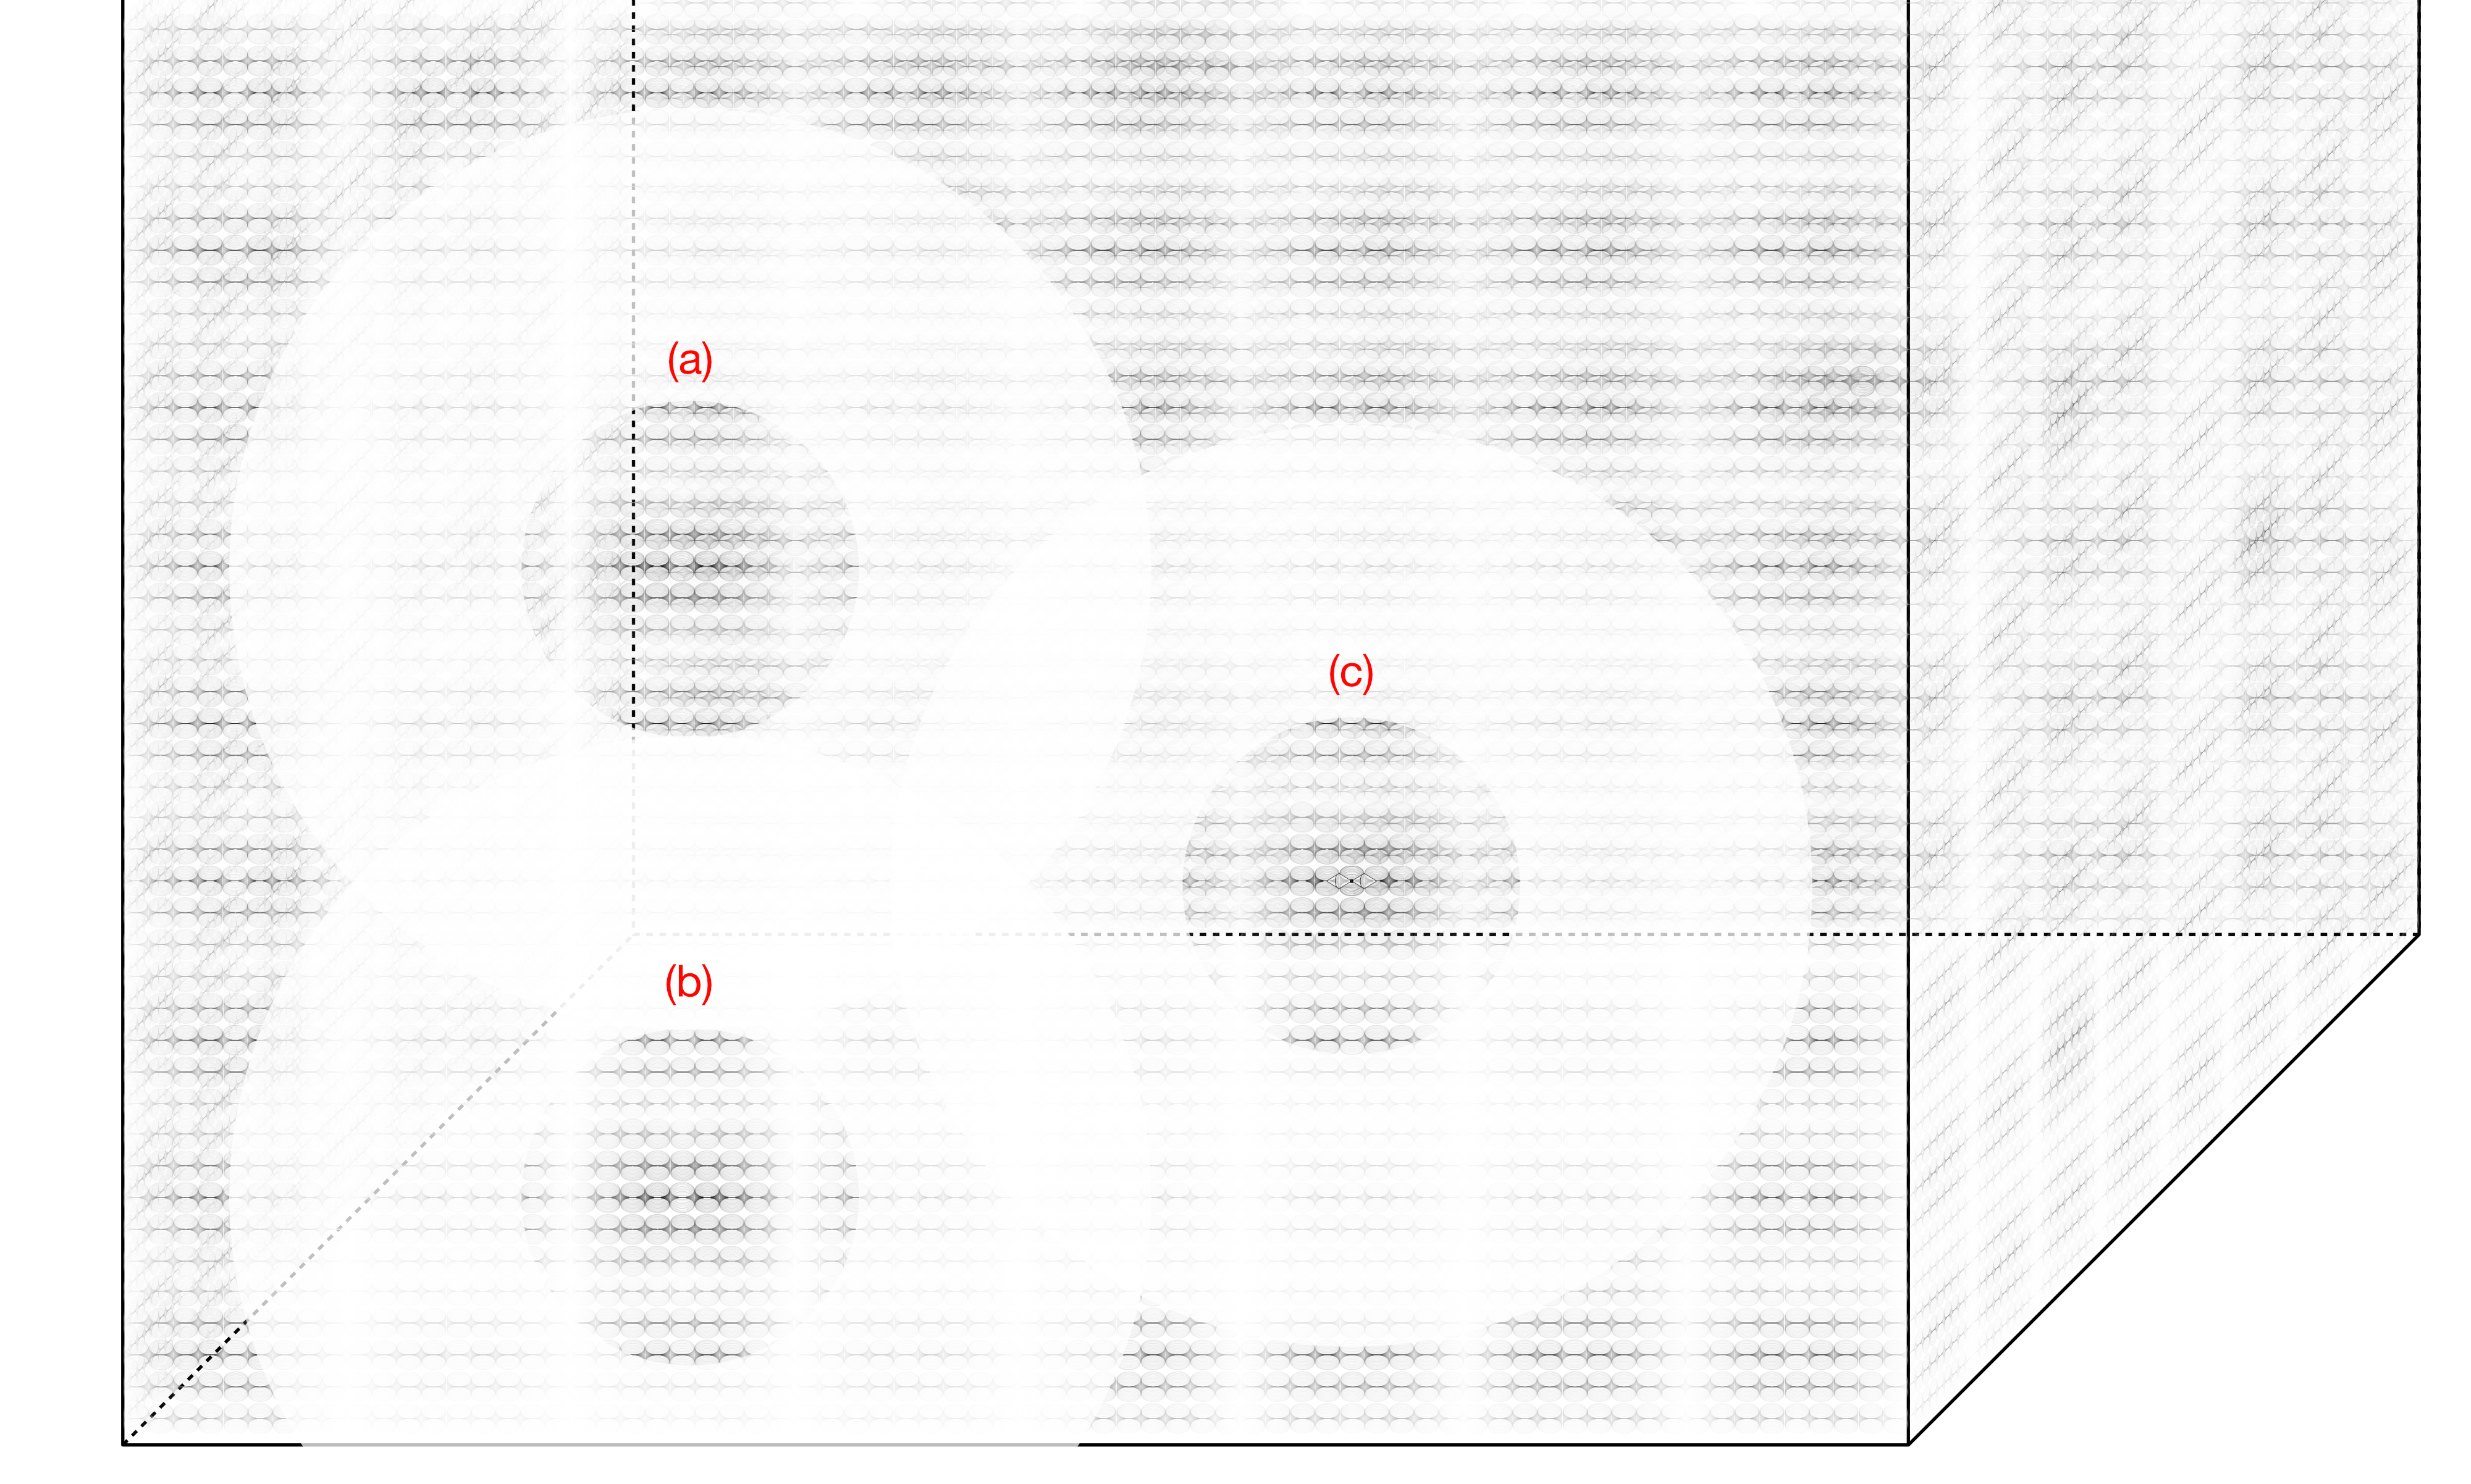
\includegraphics[width=0.7\linewidth]{figures/4.5.png}
    \caption[Larger field of horn tori as point plot heatmap]
    {\textbf{Larger field of horn tori as point plot heatmap.}}
    \label{f4.5}
\end{figure}
\FloatBarrier


\FloatBarrier
\section{Experiment to test computational information management of a hyperlinked research database}
\begin{figure}[h]
    \centering
    \includegraphics[width=\linewidth]{figures/4.6.png}
    \caption[Obsidian network graph of my research database and detail]{\textbf{Obsidian network graph of my research database and detail.}}
    \label{f4.6}
\end{figure}
\index[terms]{network graph}
\FloatBarrier

To test the production of network graphs in PKM, I began my work with Obsidian, a markdown language platform that allows users to hyperlink across text files \citep{obsidian_obsidian_nodate}. Obsidian user databases are called vaults, individual text files are called pages, bulleted lines of text are called blocks, and hyperlinks are called links. Users of Obsidian’s predecessor Roam Research \citep{roam_research_roam_nodate} or other similar platforms like Logseq \citep{logseq_logseq-_nodate} may be familiar with some of the terminology and Markdown language formatting \citep{gruber_markdown_2004, swartz_html2text_2011}. 
\index[people]{Swartz, Aaron}
\index[people]{Gruber, John}

I set up my workflow for collecting sources and linking them following courses by Danny Hatcher \citep{hatcher_become_nodate} and Lisa-Marie Cabrelli \citep{cabrelli_roam_nodate}. I consulted with Jay L. Colbert \citep{colbert_about_2022} to set up synchronization of my Obsidian and Logseq databases. 


As part of my survey of similar platforms, I tested Logseq, which drew me in with its default mode for outlining text using collapsible lists of nested bullet points. I coded a Logseq index page that automatically listed all my database blocks under letters of the English alphabet, Arabic numerals, and Adler's set of 102 syntopical terms \citep{adler_great_1952-2}. Logseq's collapsible bullets were an especially valuable user interface feature in a long index page like mine, shortening scrolling time by tucking away blocks under their category name unless I actively clicked on a letter, number, or term of interest. 


The following Markdown code shows how I listed blocks from my database which start with the letter `a':

\begin{verbatim}
#+BEGIN_QUERY
{
  :title "Pages that start with a"
  :query [
    :find (pull ?p [*])
    :where [
      [?p :block/name ?name]
      [(clojure.string/starts-with? ?name "a")]
    ]
  ]
}
#+END_QUERY
\end{verbatim}


I made my Logseq index page by modifying the string query code from Logseq discussion forum user starryvechsh \citep{noauthor_how_2022}. The full-length code for my Logseq index is available in \href{https://github.com/orusmateo}{my GitHub repository}. 

\index[people]{Adler, Mortimer J.}
\index[terms]{Syntopicon}

\section{Experiment to test topic modelling between semantic fields for interdisciplinary Knowledge Translation}

Drawing on my lived experience of being raised Roman Catholic while working towards climate crisis mitigation, I made topic models using the platform InfraNodus \citep{paranyushkin_infranodus_nodate-2}\footnote{InfraNodus uses the Louvain community detection algorithm proposed by Blondel et al. \citep{blondel_fast_2008,paranyushkin_force_2022}; InfraNodus notes in a tool-tip within the interface that its High-Level Ideas were generated using GPT-4. } of the papal encyclical \textit{Laudato si’} \citep{bergoglio_laudato_2015} and the \textit{Synthesis Report of the IPCC Sixth Assessment Report} \citep{lee_ipcc_2023} to graph intersecting themes in pursuit of Knowledge Translation across semantic fields, and to better understand both texts in relation to each other. The result included ten labels for groups of intersecting: (1) development equity, (2) environmental justice, (3) climate emissions, (4) disaster risk, (5) community development, (6) religious ethics, (7) global emissions, (8) climate resilience, (9) climate action, and (10) sustainable energy. 


\index[people]{Paranyushkin, Dmitry}
\index[terms]{InfraNodus}
\index[terms]{Knowledge Translation (KT)}
\index[terms]{climate resilience}
\index[people]{Francis, Pope}
\index[terms]{Intergovernmental Panel on Climate Change (IPCC)}
\index[terms]{Knowledge Translation (KT)}
\index[people]{Francis, Pope}



\begin{figure}[h]
    \centering
    \includegraphics[width=0.6\linewidth]{figures/4.8.png}
    \caption[Topic model of themes shared between two texts]{{\textbf{Topic model of themes shared between two texts.} Graph of themes present in both \textit{Laudato si'} \citep{bergoglio_laudato_2015} and the \textit{Synthesis Report of the IPCC Sixth Assessment Report}} \citep{lee_ipcc_2023}. Ten high-level ideas are identified here by InfraNodus and labelled in bright colours as (1) development equity, (2) environmental justice, (3) climate emissions, (4) disaster risk, (5) community development, (6) religious ethics, (7) global emissions, (8) climate resilience, (9) climate action, and (10) sustainable energy. Generated in InfraNodus and used with permission.}
    \label{fig:4.8}
\end{figure}
\index[terms]{Intergovernmental Panel on Climate Change (IPCC)}
\index[people]{Francis, Pope}
\index[terms]{climate resilience}
\FloatBarrier

\clearpage
\par
I found that there are concepts present in the \textit{Synthesis Report of the IPCC Sixth Assessment Report} but missing in \textit{Laudato si'}, and vice versa. I was concerned that ‘adaptation’ and ‘mitigation’ were not a part of \textit{Laudato si’}. Conversely, the \textit{Synthesis Report of the IPCC Sixth Assessment Report} did not include the terms `god’ and `church,’ which is unsurprising considering it is not a theological document.

InfraNodus also provided a list of entry points to develop each text, which it calls \textit{conceptual gateways}. In addition to the previous missing concepts to develop \textit{Laudato si’}, this topic model recommended developing the ideas of `infrastructure’ and `warming.’ 

While neither document fully represents climate science or theology, topic modelling across disciplines using InfraNodus was a promising example of emerging computational techniques for interdisciplinary climate text analysis.

\index[people]{Francis, Pope}
\index[terms]{Intergovernmental Panel on Climate Change (IPCC)}
\index[terms]{InfraNodus}


\begin{figure}[h]
    \centering
    \includegraphics[width=0.8\linewidth]{figures/4.9.png}
    \caption[Missing Concepts comparison]
    {\textbf{Missing Concepts comparison.} \textit{Left}: concepts in the Synthesis Report of the \textit{IPCC Sixth Assessment Report} but missing from \textit{Laudato si'}. \textit{Right}:  concepts in \textit{Laudato si'} but missing from the Synthesis Report of the \textit{IPCC Sixth Assessment Report}. Left and right Missing Concepts lists were generated under the Blind Spots tab in the Text Analytics Panels of InfraNodus, and shown side-by-side here for comparison. Used with permission.}
    \label{fig:4.9}
\end{figure}
\index[terms]{Intergovernmental Panel on Climate Change (IPCC)}
\index[terms]{InfraNodus}
\index[people]{Francis, Pope}

\begin{figure}[h]
    \centering
    \includegraphics[width=0.8\linewidth]{figures/4.10.png}
    \caption[Conceptual Gateways comparison]
    {\textbf{Conceptual Gateways comparison.} \textit{Left}: gateways for \textit{Laudato si'}. \textit{Right}: gateways for the \textit{Synthesis Report of the IPCC Sixth Assessment Report}. Left and right Conceptual Gateways lists were generated under the Blind Spots tab in the Text Analytics Panels of InfraNodus, and shown side-by-side here for comparison. Used with permission.}
    \label{fig:4.10}
\end{figure}
\index[terms]{Intergovernmental Panel on Climate Change (IPCC)}
\FloatBarrier
\index[terms]{InfraNodus}
\index[people]{Francis, Pope}

\clearpage


\section{Experiment to test more ecological local AI}
\begin{quote}
    ``\textit{The ecology of the vast symbolic world has to be supported by a material infrastructure of sustainability and responsibility, and turning our back on the real is no way to guarantee the virtual}” \citep[p. 196]{drucker_graphesis_2014}. 
\end{quote}
Since my thesis works to apply the ``studio laboratory of knowledge design” \citep[p. 197]{drucker_graphesis_2014}  and ``knowledge engineering” \citep[p. 8]{wielinga_kads_1992}  behind Sustainability Transitions Knowledge Activation, it is foundational to approach this work while managing its ecological cost. AI, in particular, has a large and growing cost that is ``widening disparity in how different regions and communities are affected” \citep{ren_uneven_2024}. 
\index[terms]{Sustainability Transitions} \index[terms]{Knowledge Activation (KA)} \index[terms]{Sustainability Transitions Knowledge Activation (STKA)} 
\index[people]{Drucker, Johanna}

Considering the environmental costs of using AI, I moved to test topic modelling using Small Language Models that can run on my local workstation. Computer scientist Rahul Nayak proposes one such solution to create what he refers to as graphs of concepts using Mistral 7B, named after its comparably small seven billion parameters \citep{nayak_how_2023}.
\index[terms]{Large Language Model (LLM)} 
\index[terms]{Small Language Model (SLM)} 
\index[terms]{Language Model (LM)} 

Software engineer Juan Sulca and I successfully used Nayak’s method to create a navigable and searchable graph of concepts of \textit{Laudato si’}. However, further development would be required to create a comparison graph such as the one generated by InfraNodus.
\index[terms]{InfraNodus}
\index[people]{Francis, Pope}

\FloatBarrier
\begin{figure}[h]
    \centering
    \begin{minipage}[t]{0.48\linewidth}
        \centering
        \includegraphics[width=\linewidth]{figures/4.11.png}
        \caption[Overview of the \textit{Laudato si'} graph of concepts]    {\textbf{Overview of the \textit{Laudato si'} graph of concepts.} Topic model made using Rahul Nayak’s Mistral 7B method \citep{nayak_how_2023}.}
        \label{f4.11}
    \end{minipage}%
    \hfill
    \begin{minipage}[t]{0.48\linewidth}
        \centering
        \includegraphics[width=\linewidth]{figures/4.12.png}
          \caption[Detailed view of the \textit{Laudato si'} graph of concepts]    {\textbf{Detailed view of the \textit{Laudato si'} graph of concepts.} Topic model made using Rahul Nayak’s Mistral 7B method \citep{nayak_how_2023}.}
        \label{f4.12}
    \end{minipage}
\end{figure}
\index[people]{Francis, Pope}

\par

\FloatBarrier

\section{Stewarding knowledge for climate resilience}
A number of political and economic factors actively detract from climate mitigation. For example, hyper-specialization is convenient for the current predominantly empire-driven capitalist extractivist economy; hyper-specialization makes humans monocrops for convenient harvesting through overwork, which keeps large populations subjugated as politically docile consumers. It seems to me that it is convenient to keep researchers underinformed about solutions from other fields that support climate crisis mitigation. This means solutions can be bought and sold to maintain control of populations. Specialization is required to achieve proficiency and make an impact in any field, but isolation-reinforced hyper-specialization does not have to be the norm.
\index[terms]{network graph}

As the earth careens toward catastrophe, resistance will inevitably ensue, and oppressors will have the prerogative to control populations by harsher means. The university context has historically facilitated resistance against the ideological and technological structures that limit climate justice and climate resilience. Discussing my research has taught me that many organizations, including universities, struggle to best use available information to facilitate researcher grouping, which significantly restricts funding for many deserving initiatives. In my pursuit of building better tools for connecting ideas, I also aim to connect the people who have them. Doing both makes it more likely that we will reveal solutions for climate crisis mitigation that may exist in the information we already have. 
\index[terms]{climate justice}
\index[terms]{climate resilience}